\documentclass[a4paper, 10pt]{report}
\usepackage[utf8x]{inputenc}
\usepackage[francais]{babel}
%\usepackage{color}
\usepackage[pdftex]{graphicx}
\usepackage{pstricks}

\renewcommand{\labelitemi}{$\bullet$}
\renewcommand{\labelitemii}{$\cdot$}

\begin{document}

\title{Implémentation d'un produit de matrices tolérant aux fautes}
\author{
Georges Abou Haydar\\\texttt{georges.abou\_haydar@etu.upmc.fr}
\and Mikael Caçote\\\texttt{mikael.cacote@etu.upmc.fr}
\and Encadrants : Jean-Luc Lamotte et Philippe Trébuchet
}
\maketitle

\begin{abstract}
Avec des gravures de plus en plus fine, les processeurs engendrent de plus en plus de fautes 
non détectées qui peuvent complètement invalider des calculs. Face à ce problème, différentes 
approches sont possibles. Dans le cadre de ce projet, nous nous intéresserons à l'approche ABFT 
(Algorithm-based Fault Tolerant) pour des algorithmes de calcul numérique et plus particulièrement 
pour le produit matriciel. La méthode s'appuie sur une extension de la taille des matrices afin de 
calculer des valeurs au fur et à mesure des calculs qui servent à vérifier l'intégrité des résultats. 
Un article fondateur de K.-H. Huang, J.A. Abraham \cite{Huang} explique son principe. 
\end{abstract}

\tableofcontents

\chapter{Principe}
\label{chap:Principe}
\section{Introduction}
\paragraph*{}
Depuis quelques années, les industriels voient monter en flèche un nouveau type de bug informatique,
provoqué par ces particules qui sillonnent l’Univers à de vitesses proches de la lumière et percutent sans
cesse la Terre. Il s'agit des rayons cosmiques.\newline
"Quand ils pénètrent dans l’atmosphère, les noyaux d’atomes et les protons, qui forment l’essentiel des
 rayons cosmiques, se désintégrent en grandes cascades de particules", décrit Jim Ziebler. Ces particules
 arrivant en contact avec un noyau de silicium peuvent créer une charge éléctrique permettant
d'inverser l'état logique d'un bit.\newline
De plus, avec la miniaturisation des circuits, la sensibilité aux rayons cosmiques a connu une forte 
croissance. Ceci est dû au fait que les courants circulant dans ces circuits deviennent de plus en plus 
faible ainsi moins d'énergie est nécessaire pour basculer des bits.
Ceci nous amène a croire que l'occurrence d'une erreur est plus probable de nos jours et que le nombre 
d'erreur à un instant t augmente à son tour.\newline 
Aucun circuit éléctronique n'est à l'abri de rayons cosmiques. Dans le cadre des ordinateurs on peut alors 
dire qu'une erreur peut subvenir dans n'importe quelle partie de l'ordinateur : le processeur, la mémoire 
vive, le bus \ldots
\paragraph*{}
Pour bien présenter le problème nous devons d'abord définir quelques termes fondamentaux nécessaires à la 
compréhension du sujet.\newline
La \textbf{sûreté de fonctionnement} d'un système permet aux utilisateurs de placer une confiance 
justifiée dans le service que délivre ce système. Cette sûreté dépend de plusieurs facteurs. Nous pouvons 
citer parmi ces facteurs la \textbf{fiabilité} et la \textbf{disponibilité} du système. La fiabilité 
repose sur le fait que le système est en état de rendre un service conforme à sa spécification alors que 
la disponibilité n'est autre que la fraction de temps pour laquelle il n'est pas défaillant et du coup 
disponible pour rendre son service.
\paragraph*{} 
Les erreurs amenées aux systèmes par des facteurs comme les rayons cosmiques, peuvent provoquer des 
défaillances et ainsi dégrader la sûreté des systèmes.\newline
Plusieurs techniques ont été développées afin d'essayer de prévenir ou d'éliminer les fautes. Elles se partagent en deux 
grandes familles : la \textbf{compensation} ou \textit{error masking} et le \textbf{recouvrement}  ou  \textit{error 
recovery}. Toutes les techniques se basent sur un principe unique : la \textbf{ redondance }.\newline
Dans le cadre de la compensation nous pouvons citer par exemple le \textit{TMR} ou \textit{Triple Modular Redundancy} qui 
s’appuie sur la redondance matérielle (en effectuant le même calcul sur 3 processeurs en parallèle) et un système de vote 
fiable pour masquer une erreur. Bien que le TMR soit une technique assez générale applicable à tous les modules, elle 
est extrêmement coûteuse au niveau matériel.\newline
Le traitement d'erreurs par recouvrement remplace l'état erroné du système par un état correct. Il se partage lui aussi
en deux catégories : le recouvrement par \textbf{ reprise } ou \textit{ backward recovery } et le recouvrement par 
\textbf{ poursuite } ou \textit{ forward recovery }. Le recouvrement par reprise essaye de ramener le système à un état 
antérieur correct. Un bon exemple serait le \textit{ checkpointing }. Il s'agit de la technique la plus connue et 
utilisée pour obtenir une tolérance aux pannes dans les systèmes critiques ou les super calculateurs comme \textit{ road 
runner } qui tourne à une moyenne de 32 pannes par jour. Elle consiste à stocker un état cohérent d'un système réparti 
d'une manière périodique et puis revenir au dernier état correct en cas de panne. Le \textit{ checkpointing } est 
efficace dans quelques cas mais souffre d'un problème de mise à l'échelle. Avec l'augmentation du nombre de processeurs
le nombre d'enregistrements devient de plus en plus important alors que ces derniers sont connus pour être le principal 
coût de cette technique. Ainsi, la disponibilité de système decroit en diminuant la sûreté du système. Or dans des 
systèmes désirant avoir une grande puissance calculatoire la disponibilité est un facteur très important.

\paragraph*{}
Dans ce projet, nous n’entrerons pas dans les détails des différentes techniques de correction d’erreurs. 
Notre but est de réussir à implémenter un système tolérant aux fautes assez léger et accessible sur n’importe 
quel ordinateur récent.
K.-H. Huang et J.A. Abraham présentent dans leur article fondateur intitulé : \textit{``Algorithm-Based 
Fault Tolerance for Matrix Operations''} \cite{Huang} un algorithme permettant de réaliser un système tolérant aux fautes 
répondant à nos besoins. Il s'agit d'une technique qui peut être classée dans la dernière famille que nous avons cité : 
le recouvrement par poursuite basé sur le reconstitution d'un état correct courant.  
\newpage
\section{Encodage et Matrices}
\paragraph*{}
Nous nous intéresserons en particuliers à la détection et la correction d’erreurs dans le calcul matriciel 
au sein du processeur (et juste le processeur). Le principe de cette technique réside sur les propriétés d’un 
\textit{checksum}. Celui-ci étant conventionnellement calculé au niveau d’un mot (dans ce cas un entier ou un flottant), 
nous ne pourrions pas détecter les erreurs affectant tous les bits du mot. Donc nous encoderons nos données à 
un plus haut niveau.\newline
Dans la représentation choisie par K.-H. Huang et J.A. Abraham, les matrices, cela serait la ligne ou la colonne
contenant les différents éléments de la matrice. Nous verrons par la suite que cet encodage permettra de localiser 
l’élément de la matrice affecté par le défaut et ceci grâce à la redondance dans l’encodage. Cette redondance est due au 
fait qu’un élément donné d’une matrice intervient dans le calcul du \textit{checksum} au niveau de la ligne et de la 
colonne dans lesquelles il se trouve. Dans le cadre de ce projet on parlera alors d’une redondance au niveau de 
l’information.
\paragraph*{}
L’encodage ou plus précisément le \textit{checksum} d’une ligne ou d’une colonne est tout simplement la somme de ses 
éléments. 
Les \textit{checksums} calculés successivement sur toutes les lignes ou colonnes forment un vecteur qu’on peut appeler 
dans ce cas un vecteur de sommation.\newline
En se servant des deux vecteurs de \textit{checksums} calculés pour chaque matrice (un vecteur de sommation pour les 
lignes 
et un pour les colonnes), nous pourrions étendre notre matrice d’information en réalisant l’une des trois combinaisons 
suivantes : 
\begin{itemize}
 \item la matrice d’information avec son propre vecteur de \textit{checksums} de ligne,
 \item la matrice d’information avec son propre vecteur de \textit{checksums} de colonne
 \item et finalement la matrice d’information avec ces deux vecteur de \textit{checksums}.
\end{itemize}
Les auteurs de l'article baptisent les matrices obtenues respectivement \textit{Row Checksum Matrix} (RCM), 
\textit{Column Checksum Matrix} (CCM) et \textit{Full Checksum Matrix} (FCM) ; en fait une FCM n’est autre 
qu’une CCM d’une RCM.
\newline
\label{sec:Matrices}
Ainsi, nous avons trois nouveaux types de matrices que nous rajoutons au type de base qui est la matrice d’information.

\section{Extensions Vs. Opérations}
\label{sec:Operations}
\paragraph*{}
Par la suite, K.-H. Huang et J.A. Abraham démontrent que 5 opérations élémentaires sur les matrices préservent 
la propriété que possèdent leurs checksums. Il s’agit des opérations suivantes : \newline
La multiplication de deux matrices, la multiplication d’une matrice par un scalaire, la décomposition $LU$, 
l’addition de deux matrices et la transposition d’une matrice.
\paragraph*{}
On retient de ces démonstrations les résultats suivants :
\begin{itemize}
 \item Le résultat de la multiplication d’une \textit{Column Checksum Matrix} $A_c$ avec une \textit{Row Checksum Matrix}
       $B_r$ est une \textit{Full Checksum Matrix} $C_f$ tel que les matrices d’informations correspondantes ne sont pas 
       affectées par l’extension (voir figure \ref{fig:mult}). Ainsi \[ A_c \times B_r = C_f \Leftrightarrow A \times B = C \]
\begin{figure}
 \center
 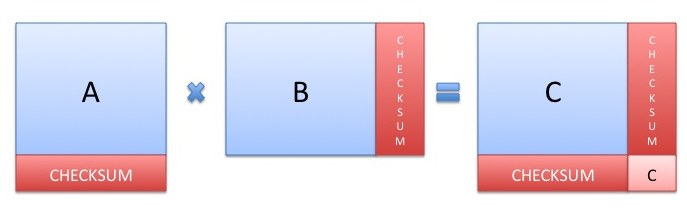
\includegraphics[scale=0.45]{Multiplication.jpg}
 \caption{Multiplication de deux matrices encodées}
  \label{fig:mult}
\end{figure}
 \item Le même théorème peut s’appliquer pour la multiplication par un scalaire. Ainsi
       \[ A_f \times x = C_f \Leftrightarrow A \times x = C \]
 \item En ce qui concerne la décomposition $LU$, Si une matrice est décomposable en $LU$ sans pivotage 
       (c.-à-d. $C = LU$) la matrice $C_f$ correspondante est elle aussi décomposable en deux matrices $L_c$ 
       et $U_r$ dans lesquelles la matrice d’information n’est autre que la matrice $L$ ou $U$ correspondante 
       dans la décomposition de $C$ (voir figure \ref{fig:lu}).
       Ainsi \[ L_c \times U_r = C_f \Leftrightarrow L \times U = C \]
       Dans ce cas seul une détection d'erreur peut \^etre effectuée sur $L_c$ 
       et $U_r$ afin d'éventuellement relancer le calcul mais les erreurs ne peuvent en aucun cas \^etre corrigées sur des matrices ne contenant qu'un
       vecteur de sommation.
       Si la matrice n'est pas décomposable sans pivotement alors elle est seulement décomposable en $C = PLU$ o\`u P est la matrice de pivotage,
       et on n'obtient plus des matrices $L_c$ et $U_r$ valides sur lesquelles on peut détecter des erreurs.\newline
\begin{figure}
 \center
 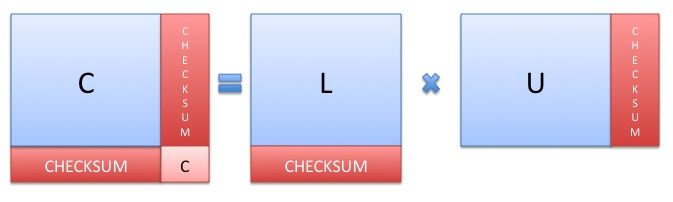
\includegraphics[scale=0.45]{Decomposition.jpg}
 \caption{Décomposition d'une matrice encodée}
  \label{fig:lu}
\end{figure}
\item Comme pour la multiplication, l’addition garde aussi le bon résultat dans la partie information de la 
      matrice résultat (voir figure \ref{fig:add}), c.-à-d. que le résultat de l’addition de deux \textit{checksum} matrices ($A_f$ et $B_f$) 
      est la matrice $C_f$ telle que :
      \[ A_f + B_f = C_f \Leftrightarrow A + B = C \]
\begin{figure}
 \center
 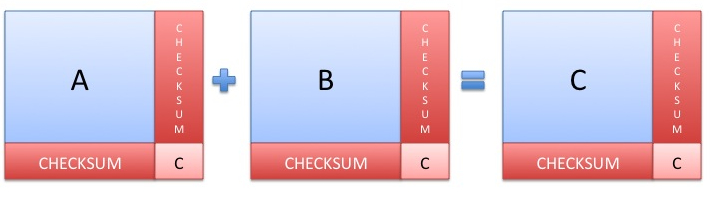
\includegraphics[scale=0.45]{Addition.jpg}
 \caption{Addition de deux matrices encodées}
  \label{fig:add}
\end{figure}
\item Et finalement après la transposition d’une \textit{Full Checksum Matrix} la matrice d’information obtenue 
      est la transposée de la matrice d’information correspondante (voir figure \ref{fig:trans}).
\begin{figure}
 \center
 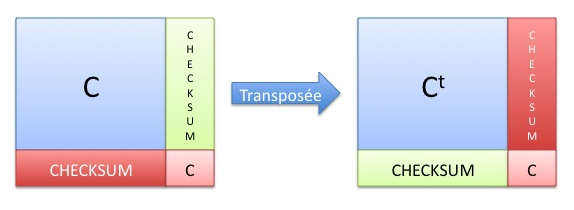
\includegraphics[scale=0.45]{Transposee.jpg}
 \caption{Transposée d'une matrice encodée}
  \label{fig:trans}
\end{figure}
\end{itemize}
\paragraph*{}
En conclusion, ces théorèmes nous permettent alors d’effectuer ces 5 opérations sans se soucier de l’influence 
que l’extension de la matrice peut avoir sur la matrice que nous étendons. En d’autres termes,  les algorithmes 
de calculs de ces cinq opérations restent inchangés s’il s’agit d’une \textit{Full Checksum Matrix}, d’une 
\textit{Row Checksum Matrix}, d’une \textit{Column Checksum Matrix} ou bien d’une matrice.\newline
Le passage d’une matrice de taille $m \times n$ à celle d’une taille $(m+1) \times (n+1)$ ne changera aucunement 
la complexité du calcul de ces cinq opérations. En effet, nous appliquons toujours le même algorithme et la taille 
de la matrice est du même ordre de la taille de la matrice d’origine.
\paragraph*{}
Pour résumer, ce que nous avons à réaliser dans notre implémentation pour l’instant, c'est de permettre le passage
d’une matrice donnée à un des trois autres types de matrices. Ensuite, la propriété du \textit{checksum} 
étant préservée, on pourra implémenter ces cinq opérations sans se soucier du type de matrice en entrée.\newline
Il reste à comprendre comment ce système de \textit{checksum}  permet, en s’appuyant sur la redondance, de détecter 
l’erreur et ensuite d’essayer de la corriger.

\section{Détection et Correction}
La question posée à ce stade serait: ``comment pourrait-t-on détecter une erreur en se basant sur cette extension ?''
Par définition l’emploi d’un \textit{checksum} a pour but principal de 
détecter l’existence d’une erreur dans l’information qu’il encode. D’ailleurs il s’agit de l’étymologie même du mot 
dans lequel ``check'' signifie vérification en anglais et ``sum'' signifie somme ou sommation.
\paragraph*{} 
Ainsi, une erreur peut être détectée dans une ligne en effectuant la somme des éléments de cette ligne 
et en comparant le résultat au \textit{checksum} de cette ligne déjà calculé suite à l’extension de la matrice vers 
une \textit{Full Checksum Matrix}. Une erreur dans ce cas correspondrait à une inégalité des deux nombres comparés. 
On détectera ainsi, que dans la ligne concernée, une erreur doit être signalée et effectivement, par la suite être traitée.
\paragraph*{}
Un problème se pose. A moins qu’il ne s’agisse d’une ligne avec un seul élément (ce qui nous intéresse pas) l’encodage 
à ce niveau pose l’inconvénient qu’une erreur dans une ligne ou une colonne ne donne aucune précision sur son
emplacement exact. Or nous avons besoin de conna\^itre celui-ci.
\paragraph*{}
Si une erreur survient dans la matrice d’information un \textit{checksum} de ligne et \textit{checksum} de colonnes 
la mettront en évidence.\newline
Considérons qu’il s’agisse d’une et une seule erreur. L’élément du \textit{checksum} de ligne ne correspondra pas 
à la somme des éléments calculés pour cette ligne, alors cette ligne contient l’erreur. De la même manière un élément 
dans le vecteur de sommation de colonne indiquera la colonne contenant une erreur. L’hypothèse sur le nombre d’erreurs 
suppose qu’il s’agit de la même erreur. On peut conclure que l’erreur se trouve alors à l’intersection des lignes et 
colonnes correspondantes.
\paragraph*{}
Les auteurs de l’article démontrent que le nombre d’éléments différents entre deux \textit{Full Checksum Matrix} différentes 
est supérieur ou égal à 4. En effet, si un élément dans la matrice d’information est modifié, pour réussir à garder 
les \textit{checksums} valides il faudra modifier au moins un autre élément dans la ligne et un élément dans la colonne de 
l'élement en question, de sorte à masquer la différence. Il faudra en plus masquer ces derniers changements. Ceci est possible
en modifiant l'élément à l'intersection de la colonne du premier changement et de la ligne du second changement. Donc les 
éléments de tout ensemble de 4 éléments appartenant deux à deux aux même lignes et même colonnes sont dépendants les uns des autres.
\paragraph*{}
On peut déduire alors que ne pouvons détecter et corriger une erreur (rappelons qu’une erreur est une modification d’un
élément dans la matrice) en supposant que les trois autres éléments avec lesquels un élément est lié restent inchangés.
La correction se base sur la redondance de l’élément de la matrice d’information dans le calcul du \textit{checksum} de 
sa ligne, de sa colonne et de la matrice entière. Après avoir détecter l’erreur à l’intersection de la ligne et de la 
colonne ou se trouve l’incohérence, pour corriger on ajoute à l’élément la différence entre la somme de la ligne ou 
colonne et le \textit{checksum} de celle-ci, par contre si l’erreur est dans le \textit{checksum} même on remplace 
l’élément erroné par la somme calculé pour sa ligne ou colonne concernée.

\chapter{Implémentation}
Après cette description détaillée du principe de l’algorithme présentée par K.-H. Huang et J.A. Abraham que nous 
appellerons par la suite ABFT (\textit{Algorithm-Based Fault Tolerance}), notre objectif principal serait de 
concrétiser cette idée et ceci en implémentant un système qui met l’algorithme en action.
\section{Choix du Langage}
\paragraph*{}
Plusieurs types de langages existent. Il faudra avant tout choisir le type de langage et puis sélectionner le langage 
le mieux adapté à nos besoins.
\paragraph*{}
Vu que nous nous intéressons seulement au calcul matriciel, nous désirons manipuler des données de type matrice. 
Alors dans ce cas, la matrice est une structure sémantique indépendante qui rassemble des données et des traitements 
sur ces données. En plus nous devons stocker l’état d’une matrice avant les calculs et son évolution au cours de 
l’exécution de ces calculs et de la correction. Nous sommes en face d’un problème nécessitant alors le \textbf{paradigme objet}.
\paragraph*{}
Mais quel langage objet choisir ? Deux langages de programmation orientés objets se présentent à l’appel : Java et C++. 
Java est issu de C++ et présente plus de sureté au niveau de la gestion de mémoire du à l’absence des pointeurs. 
Il offre le mécanisme des interfaces facilitant la tache du développeur. Par contre il est plus lent que le C++. 
Dans le cadre du développement d’un système concernant une tache aussi répétitive et bas niveau que le calcul matriciel, 
nous désirons avoir en main le langage produisant le programme le plus efficace possible. Dans ce cas \textbf{C++} répond mieux 
à notre demande et parait le meilleur choix. Nous tacherons maintenant de réaliser 
une conception qui a le gout d’être efficace tout en étant simple et logique.

\section{Conception}
\subsection{Contrats}
\paragraph*{}
Dans cette partie nous proposons de réaliser une conception du système à réaliser. Sachant que ce dernier évoluera tout 
le long du développement du projet, il faudra que la conception permette les changements avec le moindre coût. 
\paragraph*{}
Pour cela il faut définir un \textbf{contrat d’utilisation} de chaque classe. Une classe utilisera une autre via son contrat 
d’implémentation sans se soucier de la manière dont une fonction a été implémentée. Différentes classes peuvent 
implémenter le même contrat et ainsi proposer les mêmes fonctionnalités. Quand c’est le cas l’appel d’une de ces classes 
se fera à l’initialisation ou l’assemblage. Le remplacement effectué aura un impact diminué par rapport à une implémentation 
sans contrat dans laquelle une modification se propage à divers niveaux. \newline
En Java le mécanisme permettant une telle conception par contrat réside dans les \textbf{interfaces} Java. Malheureusement 
les interfaces dans le sens Java n’existent pas en C++. On sait qu’une interface en Java n’est autre qu’une classe 
abstraite pure dans laquelle aucune fonction n’est implémentée. On peut dire en quelque sorte qu’une interface au sens 
Java est une classe abstraite. Les classes abstraites étant un concept existant en C++, nous pourrions les utiliser 
pour simuler des interfaces représentant les contrats que nous voulons implémenter. Les méthodes déclarées dans cette 
classe sont toutes précédées du mot clé virtual qui fait d’elles des fonctions virtuelles permettant de les implémenter 
dans les classes filles.
\paragraph*{}
Dans nos explications nous utiliserons alors le terme interface pour qualifier ces contrats. Tout le squelette de la 
conception se fera alors à travers ces interfaces. Elles sont toutes distinguées par un préfixe \textcolor{red}{« I »} précédant leur nom. 
A chaque interface (classe abstraite) correspondra au moins une implémentation (classe concrète) du même nom sans le 
préfixe « I ».
\paragraph*{}
Notons que nous désirons obliger l’implémentation de toutes les fonctions de l’interface définie et interdire 
l’instanciation de ces interfaces sans passer par une implémentation. Ceci est possible si les fonctions que nous 
déclarons sont \textbf{virtuelles pures}. On atteint cet objectif juste en rajoutant \textcolor{red}{« = 0 »} à la déclaration de chaque fonction.

\subsection{Types Génériques}
\paragraph*{}
Les données numériques à traiter au sein du calcul matriciel sont les flottants. Par contre plusieurs choix de représentation
de flottants sont possibles. Le choix de la représentation dépend principalement de la précision avec laquelle nous voulons
stocker nos données. On peut citer les types de base : les flottants a simple precision, double précision représentant des réels
à 32 et 64 bits respectivement. Pour une précision encore plus importante il existe des bilibothèques permettant d'étendre
arbitrairement cette précision comme GMP (GNU Multiple Precision Arithmetic Library) \cite{GMP}.
Pour ne pas avoir à limiter notre système à un seul type de données, il faudra implémenter ce système pour effectuer un 
calcul sur toutes les représentations de flottants possible. Le traitement de ces données (addition, multiplication, division, etc.) est invariant. 
Il est donc inutile d’implémenter deux versions d’un objet juste pour modifier le type de données en entrée. On veut réussir 
à factoriser le code pour éviter un tel problème, et paramétrer les fonctions d’une manière permettant de lui indiquer le 
type de donnée que nous désirons traiter. Le C++ permet de résoudre ce problème grâce aux paramètres génériques
 ou \textbf{\textit{template}}.
\paragraph*{}
Nous tacherons alors à profiter des paramètres \textit{template}, des fonctions \textit{template} et des classes 
\textit{template}. Pour cela, toutes nos classes ayant une certaine relation avec les données que nous manipulons 
sont des classes \textit{template} ayant comme paramètre générique un type T qui peut être les entiers ou les flottants.\newline
La déclaration des paramètres \textit{template} se fait de la manière suivante :\paragraph*{}
\textcolor{red}{template $<$class T$>$ class nom} ou nom est le nom de la classe en question.
\paragraph*{}
Bien que le \textit{template} soit un mécanisme très pratique, il soulève un problème d’instanciation assez important. 
Les \textit{templates} doivent impérativement être définis lors de leur instanciation pour que le compilateur puisse générer 
le code de l’instance. Ceci signifie que la déclaration et la définition des différentes fonctions membres doit être réalisée 
au sein d’un même fichier. Ce qui n'est pas pratique pour la compilation séparée des différentes unités car le code source doit
\^etre inclus en m\^eme temps que la déclaration par les unités qui l'utilise. Ce qui fait que on ne profite pas de la liaison dynamique et qu'on
obtient des fichiers objets plus gros. D'autre part pour garder leur savoir 
faire certains développeurs ne désirent fournir que les déclarations de leur code à la distribution d’une bibliothèque. Par contre 
avec les \textit{templates} cela n’est pas possible étant donné que les déclarations et les définitions sont dans le même 
fichier.\newline
La solution proposée à ce problème est d’effectuer l’instanciation explicite du \textit{template} dans la partie 
définition. Cette instanciation se fait en donnant une valeur par défaut à T. On rajoute alors au fichier contenant 
les définitions « .cpp » la ligne ci-dessous si on veut instancier le \textit{template} pour des types de données réelles:\paragraph*{}
\textcolor{red}{template class NomDeLaClasse$<$double$>$;}
\subsection{Matrices}
\paragraph*{}
Nous avons conclus dans la partie \textbf{\ref{sec:Matrices}} du chapitre \textbf{\ref{chap:Principe}} que nous manipulerons quatre types de matrices dans le cadre 
de ce projet : 
une matrice sans extensions, une \textit{Row Checksum Matrix}, une \textit{Column Checksum Matrix} et finalement une 
\textit{Full Checksum Matrix}. Tous ces types de matrices ont des points communs qui forment les propriétés de bases 
d’une matrice (sans extensions), cependant présentent des différences au niveau de leurs extensions.
\paragraph*{}
Il est tout à fait naturel de vouloir créer un type d’objet pour chaque type de matrice. Ainsi nous avons créé quatre 
interfaces définissant les contrats de ces quatre objets. Vu que nous sommes dans le monde objet de C++, nous profiterons 
ainsi de l’héritage que C++ offre pour réunir les propriétés et les traitements communs dans une interface. Cette interface 
doit être la plus générale dans la hiérarchie des matrices. Celle-ci sera relative à la matrice sans extension, dans ce cas 
appelée \textbf{\textit{IMatrix}}. On remarque de même qu’une \textit{Full Checksum Matrix} est une \textit{Column Checksum Matrix} 
d’une \textit{Row Checksum Matrix}. L’interface \textbf{\textit{IFullChecksumMatrix}} peut alors hériter des interfaces 
\textbf{\textit{IRowChecksumMatrix}} et \textbf{\textit{IColumnChecksumMatrix}}.
Ainsi, nous aurons l’arbre de la figure \ref{fig:Diag1}.\newline
\begin{figure}
 \center
 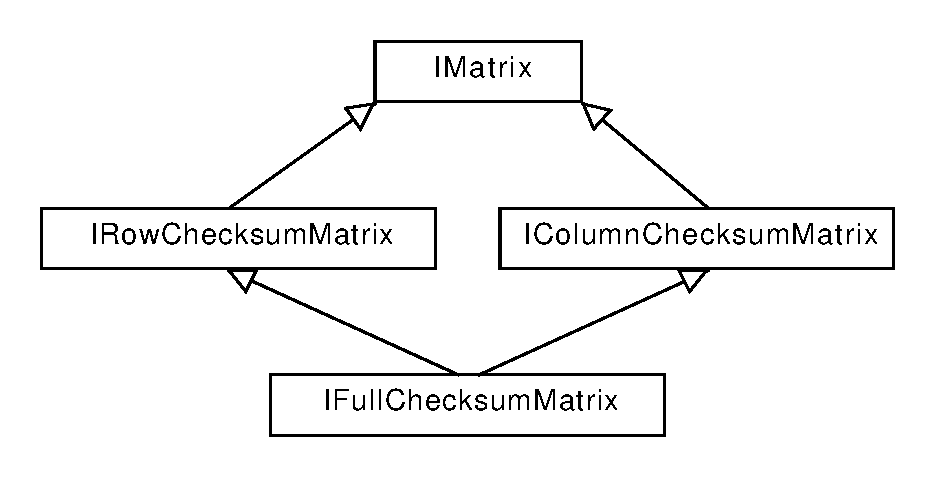
\includegraphics[scale=0.5]{MatricesHierarchie.pdf}
 \caption{Diagramme des Interfaces des Matrices}
  \label{fig:Diag1}
\end{figure}

\begin{figure}
 \center
 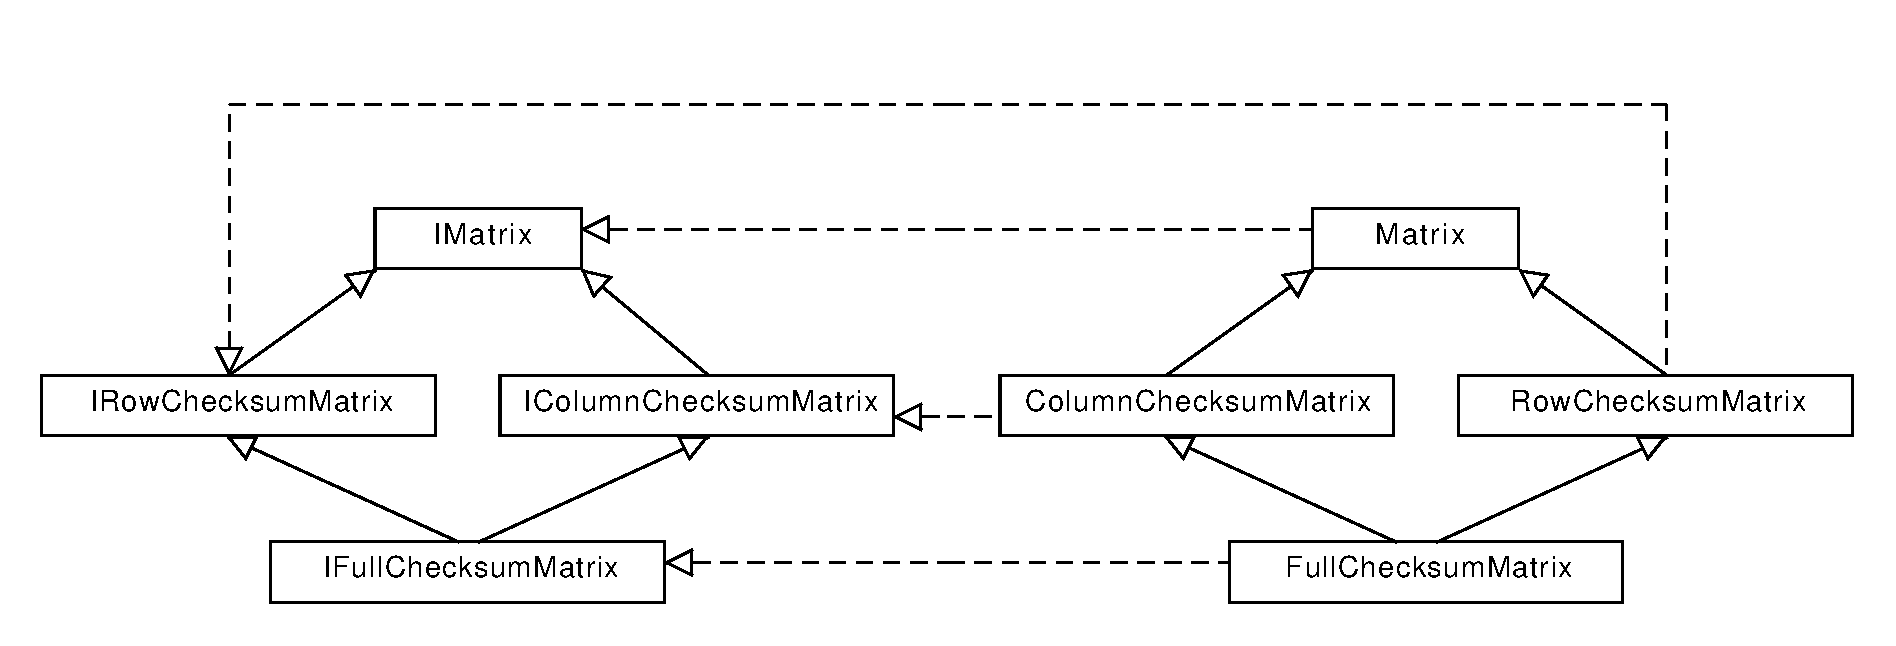
\includegraphics[scale=0.35]{MatricesHierarchie2.pdf}
 \caption{Diagramme des Interfaces des Matrices et de leurs implémentations}
  \label{fig:Diag2}
\end{figure}

\paragraph*{}
Avant de nous arrêter sur le problème que peut poser une pareille structure, nous soulignons le fait que chacune 
des interfaces sera implémentée par une classe qui respectera le contrat, ainsi dans le cas où une classe devrait être remplacée 
dans la suite du projet nous n'auront point de problèmes de compatibilité avec les autres classes.
L’arbre des classes d’implémentation de ces interfaces est calqué sur l’arbre des interfaces et nous obtenons alors, 
le diagramme de la figure \ref{fig:Diag2}.\newline
Dans ce diagramme les flèches pointillées reflètent les liens d’implémentation des interfaces, même si en C++ ce lien 
doit être le même que celui de l’héritage, nous avons voulu en faire la distinction.

\subsubsection{Le Problème du diamant}
La structure de l’arbre faite ci-dessus est dite une structure d’héritage en diamant. Elle pose quelques problèmes à la 
compilation.\newline
Vu que FCM hérite de CCM et RCM et les deux héritent à leur tour de \textit{Matrix}, FCM peut contenir deux copies des membres 
de classes \textit{Matrix} dont elle hérite indirectement (une copie des membres hérités par CCM et une autre des membres 
hérités par RCM). Quand nous faisons appel à une fonction de la classe \textit{Matrix} à partir d’une instance FCM, 
celle-ci possédant deux sous objets \textit{Matrix}, le compilateur aura un choix ambiguë à faire et ne saura alors pas
laquelle des deux choisir. Alors il signalera cette ambigüité.
\paragraph*{}
Encore une fois le mot clé \textbf{\textit{virtual}} est la solution au problème.  En utilisant \textit{virtual} dans la  
déclaration de CCM et RCM. Une seule copie de \textit{Matrix} se trouvera dans FCM, il n'y aura alors aucune ambigüité pour 
le compilateur.\newline
En effet, \textit{virtual} fait en sorte que CCM et RCM n’instancient pas \textit{Matrix} et laissent cette tache à FCM 
qui instancie sa copie de \textit{Matrix}. Cela veut dire en d’autres termes que le constructeur de FCM doit faire appel 
au constructeur de \textit{Matrix} pour que son instanciation soit complète sinon une erreur sera produite.

\subsubsection{Vecteurs de Sommation}
Toutes les matrices étendues possèdent au moins un vecteur de sommation. Pour cela, nous avons choisis de faire de 
ce vecteur un objet. Nous créons donc l’interface \textbf{\textit {IVector}} qui représentera ce vecteur. Celui-ci sera 
naturellement un champ des classes d’implémentation relatives aux interfaces des matrices étendues. Ce champ aura la 
possibilité d’être accédé et modifié dans ces classes. Un vecteur étant tout simplement une matrice à une seule colonne 
ou bien une seule ligne, \textit{IVector} héritera alors de \textit{IMatrix}.

\subsubsection{Accesseurs}
Nous avons choisi de redéfinir l'opérateur \textit{(i, j)} pour pouvoir accéder à un élément de la matrice.
Cependant un problème se pose, celui du type de retour.
Car comme nous allons le voir dans la section \ref{sec:prec} du chapitre \ref{chap:arith} le type des élément des checksums n'est pas le
m\^eme que celui des éléments de la matrice originale.
Nous devons donc définir un nouveau type \textit{TypeUnion} dont les opérateurs sont surchargés et qui contient
l'union de ces deux types, afin de pouvoir renvoyer deux types de valeurs et ceci de façon quasi-transparente.

\subsection{Processeurs et Calculs}
On sait que dans une machine les calculs sont en général effectués dans le processeur ou CPU (ou alors par un GPU).
Autre que la tache des calculs arithmétiques celui ci gère la tolérance aux fautes. Le système de tolérance aux fautes que nous réalisons est un 
système logiciel. Donc nous sommes dans l’obligation de simuler les différentes tâches du processeur : du calcul, 
en passant par la détection d’erreur, la correction de ces erreurs, arrivant même à la génération d’erreurs. Ces 
fonctionnalités sont distribuées sur tout le système. Ainsi, c’est la classe \textbf{\textit{FullChecksumMatrix}} qui 
s’occupera du test sur l’existence d’erreurs dans la matrice qu’elle encode. Si une erreur est trouvée une tentative 
de correction peut être mise en place. Cette matrice est bien le résultat d’un calcul réalisé par le processeur. 
Alors, nous implémentons les algorithmes de calculs cités dans la partie \textbf{\ref{sec:Operations}} pour réaliser les calculs sur 
les matrices. Pour cela, il faut implémenter le contrat que nous définissons dans l’interface \textbf{\textit{ICalculator}} 
de la figure \ref{fig:Diag3}.\newline
\begin{figure}
 \center
 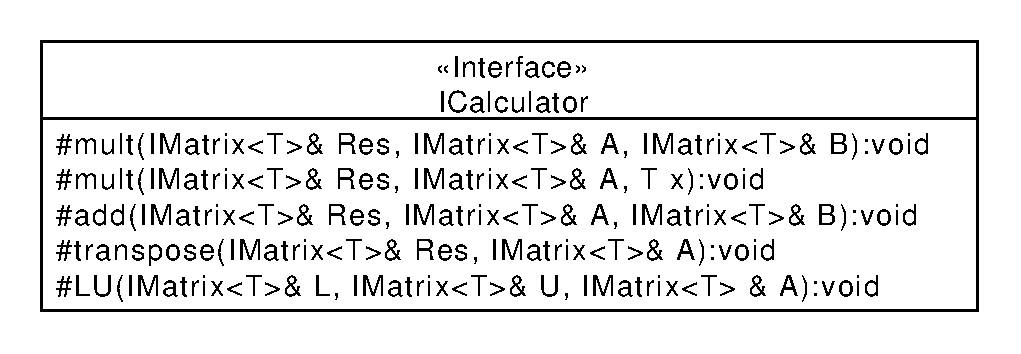
\includegraphics[scale=0.35]{ICalculator.pdf}
 \caption{Diagramme de l'interface ICalculator}
  \label{fig:Diag3}
\end{figure}
\paragraph*{}
L’implémentation de cette interface peut être effectuée de plusieurs manières. On pourra utiliser 
des bibliothèques déjà faites pour l’implémenter et ainsi profiter des propriétés et des avantages présentés 
par ces bibliothèques - Parmi ces bibliothèques nous citons \textbf{ATLAS} \cite{ATLAS}, \textbf{GotoBLAS} \cite{GotoBLAS}, \textbf{IntelMKL} \cite{IntelMKL}
ou \textbf{MPACK} \cite{MPACK} pour la précision étendue - 
ou bien essayer d’implémenter nos propres algorithmes. Puis on pourra comparer les implémentations entre-elles pour choisir 
la plus performante. Pour réaliser ceci nous devons avoir la possibilité de choisir l’implémentation que nous 
voulons à l’assemblage. Les différentes implémentations de \textit{ICalculator} auront un nom préfixé par \textit{Calculator}. 
Notre solution utilise le mécanisme de \textbf{délégation} et le patron de conception (design pattern) \textbf{\textit{Strategy}}. 
Il s’agit d’un patron de conception de type comportemental grâce auquel des algorithmes peuvent être sélectionnés à la 
volée au cours du temps d'exécution selon certaines conditions, comme les stratégies utilisées en temps de guerre d’ou son nom.
\newline
Ainsi une classe \textbf{\textit{Processor}}, dont le nom reflète la fonctionnalité se chargera du calcul matriciel sans vraiment faire 
le travail. On déclare dans cette classe un champ de type \textit{ICalculator}. Ce champ pouvant être n’importe quel 
type de calculateur on le choisit à la construction du processeur. A chaque fois que nous appelons une fonction de calcul 
dans la classe \textbf{\textit{Processor}}, celle-ci procèdera à l'extension des matrices avant de délèguer le calcul à la 
classe stockée dans ce champ qui s’occupera du reste. Puis, le processeur appellera la fonction de vérification ou 
correction d’erreurs sur la matrice résultat. La fonction de correction étant dans la classe \textit{FullChecksumMatrix} et
les fonctions de détections dans les classes \textit{RowChecksumMatrix} et \textit{ColumnChecksumMatrix}.

\subsection{Génération d'erreurs}
Bien que le vrai processeur de l’ordinateur puisse produire des erreurs, on peut attendre indéfiniment jusqu'à ce 
qu’une erreur soit produite. Cette attente n’est pas le seul problème. Si on n’est pas notifié qu’une faute a été 
induite à un calcul, on peut croire que le système que nous avons réalisé fonctionne parfaitement tant qu’aucune 
erreur n’apparait, et que ce système est systématiquement en train de corriger les éventuelles erreurs qui apparaissent 
d’une manière silencieuse. Ayant déjà simuler les calculs qu’effectue un processeur rien nous interdit de simuler la 
génération des erreurs. Si nous avons ce mécanisme en main, nous pourrions avoir le contrôle de la génération d’erreurs. 
On peut ainsi injecter une faute dans le calcul quand nous le désirons et observer la réaction du système pour traiter 
cette erreur. On peut aussi injecter un nombre d’erreurs bien précis avec des emplacements précis comme : deux erreurs 
dans la même ligne ou bien la même colonne, une erreur dans le checksum, deux erreurs aléatoires, 4 erreurs \ldots et ainsi 
de suite on peut énumérer tous les différents cas auxquels on peut penser.
\paragraph*{}
Nous choisissons alors de réaliser une interface \textbf{\textit{IErrorGenerator}} pour s’occuper de cette tâche. 
Dans cette interface nous avons une méthode \textbf{\textit{generateError()}} qui génère un certain nombre d’erreurs 
(précisé par un paramètre) dans la matrice passée en argument, dans des intervalles de lignes et de colonnes bien précises.
\paragraph*{}
Cet outil que nous implémentons est largement suffisant pour injecter des fautes dans les matrices. Pour réussir à le 
faire constamment sans arrêter les calculs, en d’autres termes faire de la génération d’erreurs simulée un événement 
vraisemblable, il faudra que son exécution s’effectue en tâche de fond.
\newline
Ceci est possible grâce à ce que nous appelons les \textbf{\textit{Threads}}. Pour présenter rapidement les \textit{threads}, 
on peut dire que c’est un mécanisme de lancement de pseudo processus légers qui partagent la même mémoire virtuelle que 
le processus principal. Leur intérêt réside dans le fait que plusieurs threads ou fils d’exécution peuvent être lancés en 
même temps. Ils s’exécutent en parallèle et communiquent entre eux grâce à l’API du langage grâce auquel nous les lançons.
La fonction de génération d’erreurs sera alors lancée pour s’exécuter en tache de fond grâce à un thread. La tache principale 
étant le calcul lui-même.

\subsubsection{Remarque  sur l’implémentation de la méthode de génération d’erreurs }
La méthode de génération d’erreurs generateError() prend 6 arguments :
\begin{itemize}
 \item \textbf{M} la matrice dans laquelle la méthode injecte l'erreur
 \item \textbf{nb} le nombre d'erreurs à générer
 \item \textbf{iMin} la borne inférieure de l'intervalle de ligne
 \item \textbf{iMax} la borne supérieure de l'intervalle de ligne
 \item \textbf{jMin} la borne inférieure de l'intervalle de colonne
 \item \textbf{jMax} la borne supérieure de l'intervalle de colonne
\end{itemize}
Les erreurs sont générées aléatoirement et itérativement dans la sous matrice déterminée par les deux intervalles de 
ligne et de colonne. Deux erreurs peuvent donc tomber à la suite dans la même case et le nombre d’erreurs que nous 
voulons injecté sera réduit de la sorte. Pour éviter ce problème nous stockons les indices des cases changés aux 
itérations précédentes.

\subsection{Tests unitaires}
La bibliothèque \textbf{CppUnit} \cite{CppUnit} à massivement été utilisée afin de tester notre code.
Elle permet d'effectuer des test unitaires pour le C++.\newline
Celle-ci est donc nécessaire pour compiler et executer notre implémentation.\newline
Les tests unitaires représentent une grande partie de ce projet : 4200 lignes de code dont 1700 lignes de tests.

\chapter{Autour de la correction d'erreur}
Nous avons déjà expliqué le principe qui réside derrière la correction d’erreurs. Cette correction utilise la propriété 
du \textit{checksum} pour détecter une erreur et profite de la redondance d’information pour tenter une correction de 
l’erreur détectée. Dans la présentation du principe nous avons considéré qu’il existe une et une seule erreur dans la matrice. 
Dans cette partie du rapport nous aborderons les différents cas présentés par la détection d’erreur. On verra que la 
correction d’une case erronée n’est autre que la solution d’un système d’équation. Nous discuterons aussi des cas ou 
la correction n’est pas certaine ou bien ne peut pas être effectuée.
\paragraph*{}
On sait que pour détecter une faute dans une ligne ou une colonne,  on calcule la somme de celle-ci et on la compare à la 
valeur du \textit{checksum} stocké dans la matrice étendue. Si les deux sont égaux alors y a éventuellement de très grandes 
chances qu’il n’ y ait pas d’erreur dans cette ligne. Cette incertitude est due au fait que plusieurs erreurs peuvent se masquer 
les unes les autres c.-à-d. que plusieurs éléments sont faux mais leur somme reste inchangée. Soit $x_1, x_2,\ldots x_n$ 
les valeurs des éléments présents dans une ligne ou bien une colonne et $c$ la valeur du \textit{checksum} de cette ligne 
ou colonne. nous devons vérifier l’égalité suivante : \[x_1 + x_2 + \ldots + x_n = c\]
Cette dernière peut être réécrite de la manière suivante : \[x_1 + x_2 + \ldots + x_n – c = 0\]
Bien que les deux écritures soient complètement équivalentes la deuxième présente un avantage important. On suppose 
qu’une erreur peut survenir dans n’importe quelle case de la matrice, les \textit{checksums} inclus. Or avec la 
première écriture on devra effectuer plusieurs tests pour savoir si l’erreur est dans le \textit{checksum} ou bien dans 
la matrice d’information, alors que l’utilisation de la deuxième ne fait aucune hypothèse sur le type de l’élément erroné. 
Quand l’égalité n’est pas respectée la ligne ou la colonne entière est considérée fausse. C’est l’intersection de cette 
ligne ou colonne avec les autres qui déterminera l’emplacement de l’erreur. L’erreur par la suite sera traitée selon cet 
emplacement facilement trouvé. S’il s’agit du \textit{checksum} on lui retranche la somme de la ligne, sinon on ajoute cette somme.
\paragraph*{}
D’une manière générale le travail consiste à résoudre un système contenant les équations des lignes et colonnes non valides. 
Le nombre d’équations est alors égal au nombre de ces lignes et colonnes et le nombre d’inconnues est celui des intersections 
entre ces lignes et ces colonnes.\newline
Déterminer le nombre de solutions pour ce système permet de discuter de la possibilité ou pas d’une correction.

\section{Une erreur}
S’il existe une seule erreur, nous avons alors une ligne et une colonne non valides. Vu que nous avons une intersection 
alors, il s’agit dans ce cas de résoudre un système de deux équations à une inconnue.\newline
Tant que le nombre d’inconnues est strictement inférieur au nombre d’équations le système a une solution unique.Donc 
dans le cas d’une seule erreur la correction est possible.

\section{Plusieurs erreurs}
\subsection{Plusieurs erreurs sur la même ligne ou la même colonne}
Soit une matrice à $m$ lignes et $n$ colonnes. Supposons que nous avons deux erreurs dans la même ligne de la matrice. 
Deux cas sont possibles :
\begin{itemize}
 \item Ces deux erreurs s’annulent : Si c’est le cas, nous n’avons pas une équation concernant une ligne erronée, par 
       contre nous avons deux équations pour des fausses colonnes. Dans ce cas il n’y a alors aucune intersection. 
       Donc le nombre d’inconnues et alors égal à deux fois le nombre de lignes de la matrices : ici $2 \times m$.
       \newline
       Le système à résoudre est un système de deux équations à $2m$ inconnues. $2m$ étant supérieure à deux alors 
       la correction dans ce cas est impossible.\newline
       Heureusement, K.-H. Huang et J.A. Abraham démontrent dans l'article que le pourcentage de détection d'une erreur 
       générée  aléatoirement dans une FCM croit très vite en fonction de la taille de la matrice vers les $99.99\%$. 
       Donc le masquage d'erreur est très peu probable.  
 \item Les deux erreurs ne s’annulent pas : Dans ce cas nous avons alors trois équations à 2 inconnues. Une équation 
       pour la ligne erronée et deux équations pour les deux colonnes erronées et une intersection entre chaque colonne 
       et la ligne (d‘ou les deux inconnues). Le nombre d’équations étant supérieur au nombre d’inconnues le système admet 
       une solution unique. On pourra corriger les deux erreurs.
\end{itemize}
Le cas de deux erreurs sur une même colonne est un cas analogue au précédent. C’est la raison pour laquelle nous ne 
le détaillerons pas.\newline
On peut généraliser ce cas pour $n$ erreurs sur une même ligne ou colonne. Supposons que les erreurs ne s’annulent pas 
alors la ligne contenant ces erreurs indique une erreur. Alors l’équation de cette ligne est une équation du système 
qu’on doit résoudre. De même les équations de $n$ colonnes ne seront pas valides. Ces équations font partie elles aussi 
du système. Le système est ainsi formé de $n+1$ équations. Chaque colonne est intersectée par la ligne qui présente l’inégalité. 
Nous avons alors $n$ intersections d’où $n$ inconnues.\newline
On sait qu'un système de $n+1$ équations à $n$ inconnues admet une solution unique. Alors dans ce cas la correction de 
la matrice est possible.

\subsection{Plusieurs erreurs sur plusieurs lignes et plusieurs colonnes}
Supposons que nous avons deux erreurs qui ne sont pas dans la même ligne ou bien la même colonne, celles-ci ne peuvent pas s’annuler. 
Alors nous aurons deux inégalités au niveau des lignes et deux autres au niveau des colonnes. Ces inégalités permettent 
alors d’avoir un système à quatre équations. Grâce aux quatre intersections entre les lignes et les colonnes en questions 
nous obtenons quatre inconnues.\newline
Ce système de quatre équations à quatre inconnues admet un ensemble de solution et non une solution unique. Quelle solution 
choisir ? Pour répondre à cette question il faudra rajouter plus de contraintes sur les données et ceci grâce à une hypothèse. 
Le choix de ces contraintes est assez subjectif mais nous essayerons de le faire d’une manière logique.
Les erreurs dans le calcul sont très peu fréquentes. Leur nombre est négligeable par rapport au nombre d’instructions 
effectuées par le processeur entre deux erreurs. Alors la probabilité d’avoir deux erreurs dans une matrice est supérieure 
à celle de quatre erreurs. Partant de ce postulat, le choix de la solution serait un choix optimal se basant sur la 
minimisation du nombre d’erreurs.
\paragraph*{}
Donc, la solution que nous proposons est la suivante :\newline
On suppose que deux des quatre éléments aux intersections sont faux. On fixe ainsi les deux autres à leur valeur dans 
la matrice (deux possibilités). On tente une correction de ces deux erreurs dans la matrice, puis on teste si tous les vecteurs de sommation 
des lignes et des colonnes correspondant à ces éléments sont valides. Si ce n'est pas le cas on effectue le même travail mais cette fois-ci
en fixant des triplets d'éléments (quatre possibilités). Dans tous les cas, on 
s'arrete à la premiere correction valide et celle-ci sera probablement la bonne.
Mais le "probablement" nous dissuade de le faire car le remède pourrait \^etre pire que la maladie.

\subsection*{}
Nous pouvont ainsi conclure que la technique nous permet de corriger jusqu'a $n$ erreurs sur la même ligne
ou $m$ erreurs sur la même colonne mais pas sur plusieurs lignes ou colonnes simultanément.

\chapter{Arithmétique flottante}
\label{sec:arith}

\section{Représentation des flottants}
La norme IEEE 754 spécifie deux formats de nombres en virgule flottante et les opérations associées.
Les deux formats fixés par la norme IEEE 754 sont sur 32 bits (simple précision) et 64 bits (double précision).
Les nombres à virgule flottante sont caractérisés pas un signe $S$, une mantisse $M$ et un exposant $E$.
Le format est décrit sur la figure \ref{fig:IEEE754} (avec $1 \preceq M \prec 2$).
\begin{figure}
\center
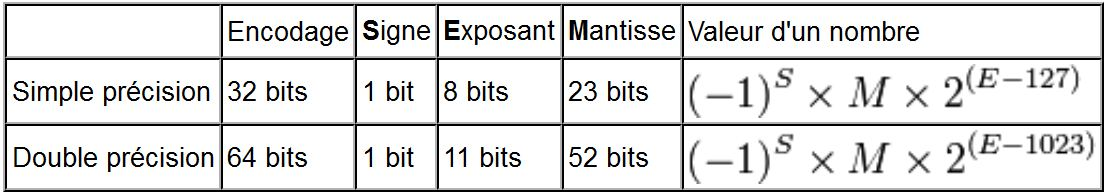
\includegraphics[scale=0.5]{IEEE754.jpg}
\caption{Flottants IEEE 754}
\label{fig:IEEE754}
\end{figure}

\section{Test d'égalité}
Pour compenser le manque de précision dû aux nombres non représentables sur le coeur de la matrice résultat on utilise un test d'égalité avec une marge de tolérance
qui est basée sur la représentation des flottants IEEE 754 et l'ordre lexicographique \cite{float} qu'il est possible d'obtenir en les transformant en entier (deux entiers pour les doubles).\newline
Cette technique est meilleure que les comparaisons avec un epsilon absolu ou relatif, car elle utilise l'univers des flottants représentables.\newline
En effet il est beaucoup plus judicieux de dire qu'on autorise une marge d'erreur de $n$ flottants avant ou après, que d'avoir une marge d'erreur en valeur qui n'utilise
pas le fait que beaucoup ou non de flottants sont représentables dans cette plage (le format implique que plus on se rapproche de 0, plus le nombre de flottants représentables est grand).\newline
Nous avons adapté cette technique aux doubles ce qui nous permet d'obtenir deux epsilons qui sont des entiers sur 32 bits, et une bijection entre deux entiers et un double.

\section{Précision des checksums}
\label{sec:prec}
Nous remarquons que le nombre d'erreurs détectées est parfois plus grand que le nombre d'erreurs réelles.
Ceci est dû à la taille des conteneurs des valeurs des éléments et surtout à la valeur du \textit{checksum} qui ne
correspond pas toujours à la somme de sa ligne ou sa colonne. Les flottants sont stockés sur un certain nombre de bits, alorser
si jamais un nombre doit etre stockée sur plus de bits sa valeur est tronquée (suivant un certain mode d'arrondi) et ne correspond donc plus à la vrai
valeur calculée. On dit alors que la valeur n'est pas représentable par un flottant de cette taille\newline
Par exemple, dans un calcul en flottants IEEE double précision, $(2^{60}+1)-2^{60}$ ne donne pas 1, mais 0. La raison est que 
$2^{60}+1$ n'est pas représentable exactement et est approché par $2^{60}$.\newline
Si la valeur est plus grande que la plus grande valeur représentable, on parle d'\textit{overflow}.
Et si elle est entre 0 et la plus petite valeur représentable, on parle d'\textit{underflow}.
\paragraph*{}
Pour contourner ces problèmes lors de la sommation des lignes et des colonnes, il suffit d'accorder plus de bits aux checksums.
Nous avons donc utilisé une bibliothèque de calcul multi-précision pour stocker les checksums
et les calculs intermédiaires.
La solution retenue est la bibliothèque \textbf{GMP (GNU Multiple Precision Arithmetic Library)} \cite{GMP}.
\paragraph*{}
Nous devons donc maintenant utiliser une bibliothèque implémentant le BLAS pour des calculs multi-précision (impliquant les checksums).
\textbf{MPACK} \cite{MPACK} a été la solution retenue.

\chapter{Tests de performances}
\label{sec:benchmark}
Les tests de performances ont été effectués pour le produit de deux matrices de taille $n \times n$.\newline
Les différentes librairies ont pu \^etre appelées durant la m\^eme exécution gr\^ace à la \textit{libc} et à la fonction de chargement dynamique
de librairies partagées \textit{dlopen()} et assimilées.\newline
En ce qui concerne les mesures temporelles, celles-ci ont été effectuées en utilisant la fonction \textit{gettimeofday()}.

\section{Matériel utilisé}
Une machine virtuelle simple coeur avec 1Go de mémoire vive a été utilisée pour illustrer le peu de ressources nécessaires à l'utilisation de la technique.\newline
Une machine récente avec une architecture multi-coeurs aurait montré des performances largement meilleures mais n'aurait pas rendu les tests de performances plus parlants
sur le co\^ut de la technique.

\section{Les différentes implémentations du BLAS}
Le Basic Linear Algebra Subprograms (BLAS) est un ensemble de fonctions standardisées (interface de programmation) réalisant des opérations de base de l'algèbre linéaire comme des multiplications de vecteurs ou de matrices. Largement utilisées pour le calcul haute performance, ces fonctions ont été implémentées de manière très optimisée.\newline
La très célèbre fonction \textit{dgemm} est utilisée par notre implémentation et représente le produit matriciel sans l'utilisation de la technique de correction d'erreurs.

\section{La technique ABFT \cite{Huang} que nous avons implémentée}
Trois étapes sont nécessaires :
\begin{itemize}
\item L'extention de la matrice originale : le co\^ut représente celui de la sommation
\item Le produit : le co\^ut représente celui du calcul de la matrice résultat et de ses checksums
\item La detection/correction : le co\^ut représente celui de la sommation
\end{itemize}

\subsection{Checksums doubles}
Ici le surplus de mémoire nécessaire est négligeable en comparaison à la mémoire utilisée par la matrice originale (de l'ordre de $n + m$).

\subsection{Checksums GMP}
\subsubsection{Calcul des checksums résultats en utilisant l'algorithme naïf (multi-precision)}
Ici le calcul du coeur de la matrice résultat est effectué par \textbf{ATLAS} \cite{ATLAS},
et le calcul des checksums résultats par l'algorithme naïf qui permet d'effectuer des calculs avec plusieurs types
sans allouer de mémoire supplémentaire.\newline
Surco\^ut en mémoire toujours négligeable (de l'ordre de $n + m$ mais avec une plus forte constante que pour les checksums doubles).

\subsubsection{Calcul de toute la matrice résultat en utilisant \textbf{MPACK} \cite{MPACK}}
Le produit est effectué en convertisant les doubles de la matrice d'information en types étendu et en appliquant la fonction \textit{rgemm}
avant de convertir le coeur de la matrice résultat en doubles.\newline
Surco\^ut en mémoire important (de l'ordre de $n \times m$).


\chapter*{Conclusion}
\addcontentsline{toc}{chapter}{Conclusion}
Nous avons abordé dans ce rapport, d'abord le principe de l'ABFT \cite{Huang} présenté par K.-H. Huang et J.A. Abraham. Ensuite, nous avons
discuté de nos choix d'implémentation de cet algorithme partant du choix du langage, en passant par la conception par contrats,
les types génériques et la simulation de génération d'erreurs ainsi que les solutions possibles au problèmes que nous pose cette
implémentation comme le patron de conception \textit{Strategy}, et les fonctions virtuelles pures. Enfin, nous avons étudié en 
détail la capacité de cet algorithme à détecter et à corriger les erreurs.
\paragraph*{}
Cette dernière partie reflète les limites de cette méthode. Ainsi on peut corriger avec certitude seulement une erreur,
cependant la correction concernant deux erreurs dépend de plusieurs facteurs dont certains que nous avons fixé pour permettre
cette correction. Il s'agit de la limite de l'utilisation des propriétés du \textit{checksum}.
\paragraph*{}
Le code source et disponible sur le site \textbf{http://pstl2010sujet9.googlecode.com/} et il peut \^etre récupéré avec la commande\newline
\textbf{svn checkout http://pstl2010sujet9.googlecode.com/svn/trunk/ pstl2010sujet9-read-only}

\begin{thebibliography}{1}

\bibitem{Huang}
KUANG-HUA HUANG, MEMBER, IEEE, AND JACOB A. ABRAHAM,
Algorithm-Based Fault Tolerance for Matnx Operations.
IEEE TRANSACTIONS ON COMPUTERS,
VOL. c-33,
NO. 6,
June 1984.

\bibitem{CppUnit}
CppUnit,
http://sourceforge.net/projects/cppunit/.

\bibitem{ATLAS}
ATLAS (Automatically Tuned Linear Algebra Software),
http://math-atlas.sourceforge.net/.

\bibitem{GotoBLAS}
GotoBLAS2,
http://www.tacc.utexas.edu/tacc-projects/.

\bibitem{IntelMKL}
Intel® Math Kernel Library (Intel® MKL),
http://software.intel.com/en-us/intel-mkl/.

\bibitem{MPACK}
The MPACK : Multiple precision arithmetic BLAS (MBLAS) and LAPACK (MLAPACK),
http://mplapack.sourceforge.net/.

\bibitem{GMP}
GMP (GNU Multiple Precision Arithmetic Library),
http://gmplib.org/.

\bibitem{float}
Bruce Dawson,
Comparing floating point numbers,
http://www.cygnus-software.com/papers/comparingfloats/comparingfloats.htm.

\end{thebibliography}

\end{document}
